\documentclass[a4paper]{scrartcl}
%preambulo

\usepackage{fullpage}
\usepackage{lmodern}
\usepackage[spanish,activeacute]{babel}
\usepackage[T1]{fontenc}

\usepackage{xcolor}

\usepackage{graphicx}

\usepackage{minted}
\newcommand{\BashFancyFormatLine}{%
  \def\FancyVerbFormatLine##1{\$\,##1}%
}

\title{SSH\_SCP Y SFTP\_V01}
\author{Facundo Navarro}

\begin{document}

\maketitle

\section{SCP}
El comando \textit{scp} (secure copy) es un comando que permite copiar de forma segura y encriptada entre un sistema local y un sistema remoto, o entre dos sistemas remotos. Se pueden realizar las siguientes operaciones:
\begin{itemize}
	\item Copiar un archivo o directorio del sistema local a un sistema remoto.
	\item Copiar un archivo o directorio del sistema remoto a su sistema local.
	\item Copiar un archivo o directorio entre sistemas remotos desde su sistema local. 
\end{itemize}

La forma gen'erica del comando scp es:
\begin{minted}[formatcom=\BashFancyFormatLine]{bash}
ssh [-option] <origen> <destino>
\end{minted}

El comando \textit{scp} requiere autentificaci'on, se debe tener una cuenta o una clave p'ublica en el sistema de destino, y asegurarse de tener al menos permiso de lectura en el sistema de origen y permiso de escritura en el sistema de destino.

\subsection{Especificaciones del origen y el destino para la copia}
Se puede especificar el origen (el archivo o direcotorio que se copiar'a) y el destino (la ubicaci'on en la que se copiara el archivo o directorio). Por parte del cluster Navira, los directorios de destino se encuentran en \textit{/home/usuario}. Las siguientes secuencias para copiar un archivo \textit{"prueba.sh"} desde el sistema local hacia el remoto son equivalentes:

\begin{minted}[formatcom=\BashFancyFormatLine,breaklines]{bash}
scp -P 2230 /home/operador/prueba.sh fnavarro@navira.cidie.ucc.edu.ar:/home/fnavarro
scp -P 2230 $HOME/prueba.sh fnavarro@navira.cidie.ucc.edu.ar:/home/fnavarro
scp -P 2230 ~/prueba.sh fnavarro@navira.cidie.ucc.edu.ar:/home/fnavarro
scp -P 2230 prueba.sh fnavarro@navira.cidie.ucc.edu.ar:/home/fnavarro
\end{minted}

Los anteriores comandos de bash son equivalentes siempre y cuando \textit{"prueba.sh"} este en \textit{/home/operador} y el comando ssh se ejecute estando en dicho directorio, lo que expone que el car'acter de tilde \textcolor{blue}{\textasciitilde} y el alias \textit{\$HOME} representa el directorio \textit{home} del usuario logueado.

\begin{figure}[ht]
	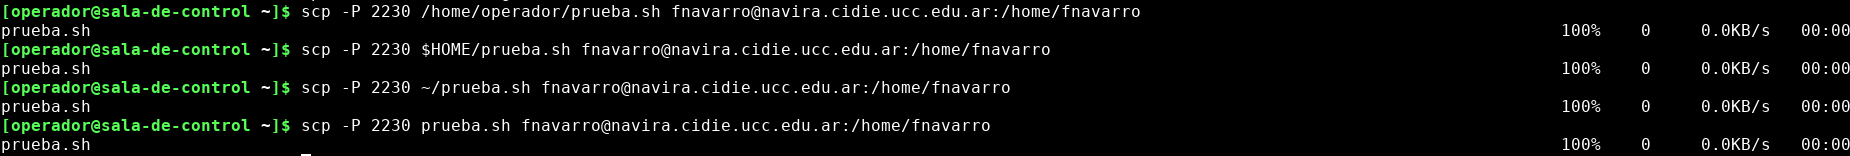
\includegraphics[width=\columnwidth]{./ssh_scp_sftp_imgs/samescp}
	\caption{Equivalencias de expresiones de PATH's}
	\label{fig:samescp}
\end{figure}

\subsection{Copiar archivos de LOCAL a SERVIDOR}
Si queremos copiar el archivo \textit{localfile.sh} de nuestro ordenador a la carpeta \textit{/home/usuario} del cluster, hacemos lo siguiente
\begin{minted}[formatcom=\BashFancyFormatLine,breaklines]{bash}
scp -P 2230 localfile.sh fnavarro@navira.cidie.ucc.edu.ar:/home/fnavarro
\end{minted}

\begin{figure}[ht]
	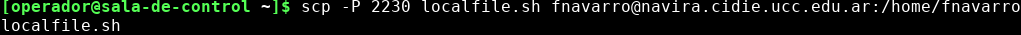
\includegraphics[width=\columnwidth]{./ssh_scp_sftp_imgs/LtoS}
	\caption{Copiando desde nuestro ordenador al Cluster}
	\label{fig:LtoS}
\end{figure}

\begin{figure}[ht]
	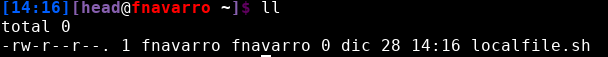
\includegraphics[scale=0.5]{./ssh_scp_sftp_imgs/LtoS_A}
	\caption{Archivo copiado en home del usuario fnavarro en el Cluster}
	\label{fig:LtoS_A}
\end{figure}

\subsection{Copiar de SERVIDOR a LOCAL}
Para traer archivos o directorios del Cluster hacia nuestro ordenador, como pueden ser los resultados de la ejecucion de los scripts, para copiar un archivo \textit{.out} del Cluster hacia el directorio \textit{home} de nuestro ordenador se realiza de la siguiente manera:
\begin{minted}[formatcom=\BashFancyFormatLine,breaklines]{bash}
scp -P 2230 fnavarro@navira.cidie.ucc.edu.ar:/home/fnavarro/slurm-191.out $HOME
\end{minted}

\begin{figure}[ht]
	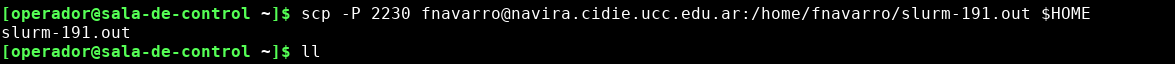
\includegraphics[width=\columnwidth]{./ssh_scp_sftp_imgs/StoL}
	\caption{Trayendo archivos desde el Cluster hacia nuestro ordenador}
	\label{fig:StoL}
\end{figure}

El mayor incoveniente de este m'etodo es tener que saber tanto el PATH completo del archivo o directorio que se quiere copoar como as'i tambi'en su nombre exacto, esto se facilita notablemente usando en vez de \textit{scp} el comando \textit{sftp} que se desarollar'a posteriormente.

\end{document}

